\documentclass[twocolumn]{ltjsarticle}
\usepackage{dcolumn}
\usepackage{pdfpages}
% 受付日などを消す
\makeatletter
\def\@uketsuke{}
\def\@euketsuke{}
\def\SHUBETUname{}
\makeatother
% ページ番号を消す
\pagestyle{empty}
\begin{document}
\title{\bf\vspace{-3cm}
{トレーディングカードゲームにおける
\\初期手札枚数差による勝率変化調査} 
}
\author{\vspace{-1cm}髙橋昇太 
阿原一志}
\date{}
\twocolumn[
\maketitle
\small{\textbf{概要:}トレーディングカードゲーム(TCG)には,手札枚数や個々のカードの攻撃力など様々なパラメータが存在する.
一般にこれらの値は勝敗に大きく関わるとされているが,科学的実証は報告されていない.
そこで本研究では,パラメータ変更による勝率の変化についてサンプリング手法を用いた調査をする.%手法の提案を行う.%変更した  
%言葉作っちゃってもいい。標本的
本論文では特に,初期手札の枚数差を意図的に生じさせ,どのように勝率が変化するかを調査した.
その結果,初期手札枚数が多いプレイヤーは勝率が高くなる傾向が明らかになった.
}
\small{
  \\
  \textbf{キーワード:}不完全情報ゲーム,トレーディングカードゲーム(TCG), ゲーム人工知能
}
\begin{center}
  \vspace{0.3cm}
\large \textbf{A Study on the Effect of the Number of Cards in the Starting Hand
  \\on the Winning Percentage in Trading Card Games
  }
\author{\textrm{
  \vspace{0.1cm}\\Shota Takahashi
  Kazushi Ahara}
  \vspace{0.1cm}
}
\end{center}
\small{\\\textbf{Abstract:}In trading card games (TCG), there are various parameters, such as the number of cards
in players' hands and the attack power of each card. Although we generally consider these values to
play essential roles in winning or losing, little quantitative evidence has been researched. In this
study, we propose a method to investigate the change of winning rate by changing parameters. This
paper examines how the winning rate changes by intentionally changing the number of starting cards
in their hands. As a result, we find that the player with more starting cards has significantly higher
winning percentages.%あとで書き直しまする
\\
\noindent
\textbf{Keywords:}Imperfect Information Game, Trading Card Game(TCG),Game Artificial Intelligence
\vspace{0.5cm}
}]
\section{はじめに}
\small{
  トレーディングカードゲーム(以下,TCG)とは「Magic: the Gathering」などを例とする2人用不完全情報ゲームで,
  近年では「Hearthstone」や「Shadowverse」のようにオンライン上で遊べるものもあり,その裾野が広がっている.%TCGのざっくりとした説明、流れを入れるとより分かりやすくなるかも
  TCG は囲碁や将棋のようにターン制で進むが,使用するカードを各プレイヤーが選べ(使用するカードの束をデッキと呼ぶ),
  デッキからランダムに引くカードの種類,いわゆる「引き」により戦局や戦略が左右されるという点がTCGの大きな特徴である.
  ここで,大まかなTCGの流れを説明する.%変更した!ここチェックして欲しいです.
  ゲームを始める際,お互い用意したデッキからそれぞれ手札としてカードを一定枚数引く.これを初期手札と呼ぶ.
  その後はルールに基づきゲームを開始する.ターンの最初に山札から1枚カードを引き,ルールにのっとり手札のカードを使用し,先に勝利条件を達成したプレイヤーの勝利となる.

  TCGには様々なパラメータが存在する.
  手札の枚数やターン数,出したカードの攻撃力値やプレイヤーの体力,デッキの枚数などがそれにあたる.
  これらのパラメータの値は対戦結果に大きな影響を及ぼすとされている.
  実際にTCG運営会社は,試合中のパラメータを考慮してルールやカード能力を設定している.%ここちょっとキモイので変更
  例えば「Hearthstone」では,先手後手の有利差を少なくするためにコインというパラメータ調整カードを後手プレイヤーに初期配布するというルールになっている.
  同様の理由で「Shadowverse」では,先手プレイヤーは手札を 4 枚,後手プレイヤーは手札を 5 枚から試合開始となる.
  またこれらのゲームでは,特定のカードやデッキの使用率,勝率が著しく高かった場合,ナーフと呼ばれるカード能力の下方修正が行われるケースもある.
  逆に,使用率の高くないカードやデッキ群に対しては,アッパーと呼ばれるカードの上方修正が行われる事もある.%この一文いるかな?
  このように,パラメータの値は試合結果に大きな影響を及ぼすことがわかっている.
  一方でこれらの事象(調整ルールやナーフ,アッパー)は経験から来る考えであると筆者は考える.
  なぜならば,TCG運営会社による定量的な検証方法などは公開されておらず,科学的実証も報告されていないためだ.

  そこで本研究では,意図的なパラメータの変更による勝率変化を,サンプリング手法を用いた実験により測定した.%ハンディキャップを生じたかどうかは書く必要なくない?
  この調査により,パラメータが試合に与える影響をより具体的な数値で観察できる.%変更した
  これは,カード能力調整をはじめとした運営開発に貢献できるほか,TCG 初心者へ向けた良質なハンデ調整などに応用できるようになると筆者は考える.
  本論文では,種種のパラメータの中から特に初期手札の枚数差による勝率変化について詳細に記す.
}
\section{関連研究}
\small{
  \verb#[1]#では,カード間の相性測定の提案並びにその有効性について実験を行った.
  相性の数値化による比較は,パラメータの比較と関連があり,今後の実験において検証する要因になりうる.

  \verb#[2]#ではMagic:The Gatheringにおいて,お互いにデッキの構成がわかっている場合,モンテカルロ木探索(MCTS)とDeterminizationを用いることが有効な手法であることを明らかにした.
  本実験でも,この手法を参考にプレイヤーエージェントの作成を行った.
}
\section{システム説明}
\small{
  本研究の実験は,Hearthstoneのシミュレーションエンジンであるfireplaceを基に,筆者らが独自に改良を加えたfireplaceAharalab[3]を用いた.
  このシミュレーションエンジンは,2019 年のHearthstone通常プレイのルールに沿って実装したもので,ハンター,ドルイド,メイジ,ニュートラルカードの 95\%以上のカード効果を再現した.
  これにより,Hearthstoneのルールを基にした汎用的なプレイの実験が可能である.
}
\section{評価実験}
\small{
  本実験では,標本標準偏差を出すためにサンプリング手法を用いた調査をした.
  以下にその手法を解説する.

  同じアルゴリズムを持つ2つのプレイヤーエージェントAとBを用意する.
  Aの初期手札は4枚,Bの初期手札は 4+α枚とする.
  ここでαを枚数差と呼ぶことにし,αは1≦α≦5の整数であるとする.
  αの範囲は,ゲームのルール上手札の枚数の上限が10枚であることを考慮し,最初のターンに上限を超えない範囲を指定した.
  本実験ではプレイ環境の違いを顕在化させるため,使用したデッキはAとBともに同じデッキである.
  AとBは1セット30戦として,これを各枚数差ごとに30戦×10セット分試合を行う.%10セット行う.%直さなくてもええか?
  本実験で使用するプレイヤーエージェントはAとBともにVectorエージェントである.
  これは,自身の体力や相手の場にいるカードの攻撃力などいくつかのデータを取り出し,
  これらの重みづけ和によって,一手読みを実行し,その結果最も良い点数の行動を行うエージェントである.
  試合開始時に行われる手札交換(マリガン)は行わない.
  先攻後攻は,先行後攻に関わらない勝率を出したかったためランダムに決定した.
  ハースストーン特有のコインは使用しない事とした。同条件下において差が生じるかを検証するためである。
  実験の結果に対し平均勝率と分散を計算し,実際に初期手札枚数差による勝率変化を見る.
}
\section{結果と考察}
\small{
  実験結果を以下に示す.
}
\begin{table}[h]
  \centering
  \caption{初期手札枚数差によるBの1セットあたりの平均勝利数と分散}
  \begin{tabular}{clll}
    α &平均勝利数(勝)& 分散\\
    \hline \hline
    \centering
    1&\multicolumn{1}{c}{16.50}&\multicolumn{1}{l}{15.17}\\
    2&\multicolumn{1}{c}{16.70}&\multicolumn{1}{l}{6.01}\\
    3&\multicolumn{1}{c}{20.10}&\multicolumn{1}{l}{3.88}\\
    4&\multicolumn{1}{c}{22.30}&\multicolumn{1}{l}{12.23}\\
    5&\multicolumn{1}{c}{22.30}&\multicolumn{1}{l}{2.21}\\
    \hline%小数点でそろえたいいいいい怒
  \end{tabular}
\end{table}
%図を入れます
\begin{figure}[h]
  \centering
  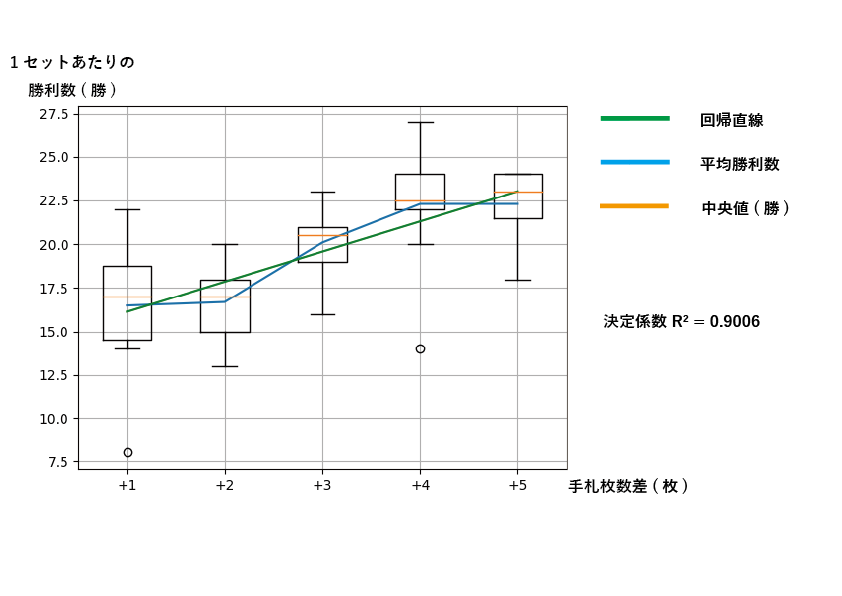
\includegraphics[scale = 0.3]{graph1.png}
  \caption{AとBの手札の枚数差とBの勝利数の箱ひげ図}
%  \label{piyo}
\end{figure}
\small{
\\
表1は,αの値による平均勝率と分散をまとめたものである.
αが大きくなるにつれて分散が小さくなり,高い勝率を維持できることが分かった.
また,図1はAとBの手札の枚数差とBの勝利数を箱ひげ図で表し,回帰直線と平均勝利数,決定係数を表示したものである.
手札枚数差と勝率の相関係数は0.943と非常に高く,手札枚数差が大きくなるほどBが勝つ傾向が見られた.
次にこの結果に至った経緯を考察する.手札が多いことのメリットとしてプレイ行動の選択肢の多さが挙げられる.
今回の分散と相関係数の結果から,手札が多くなるほど安定して勝利数が増えることが観察された.
これは,選択肢が多いと状況に応じた柔軟なプレイができ,より安定した戦略で対戦を進めることができると考えられる.
特に,αが4から5にかけて分散がより小さくなっていた.
このことから,一定の初期枚数差があるとより顕著に勝利しやすくなることが考えられる.
また,回帰直線の傾きが0.57であることから,初期枚数1枚の増加につき0.5 勝分の平均勝率の上昇が見込める.
このことから,初期枚数の違いによる有利さを定量化することができたと考えられる.
}

\section{議論と結論}
\small{
  本論文は,初期手札枚数差と勝率の関係について実験及び考察を行った.
  その結果,同様なプレイヤーであれば,初期手札枚数が多い程ゲームに安定して勝つことが分かった.
  また,この結果からTCGのパラメータ変更において,ハンディキャップの定量化ができたといえる.
  つまり,他のパラメータの差も,同様の実験で検証することができると筆者は考える.
  一方で議論すべき問題点もある.第一に,片方のプレイヤーにしか手札を増やして実験していない点である.
  実際のTCGでは,一部例外はあるものの,カードのルールによってお互いに手札を増やしながら対戦することが想定される.
  今後,手札枚数による調査を行うときは,両プレイヤーの手札を増やしつつ手札枚数差がある際の勝率を観測することも検討すべきである.
  また,本実験では手札枚数差を生じさせたのは対戦開始前であった.手札枚数差を生じさせるタイミングを変更した場合の実験も検討が必要である.
  \\第二に,特定のデッキ,プレイヤーエージェントを固定して実験を行った点である.
  プレイヤーごとに異なるデッキ,エージェントを用いても同様の結論は見込めるものの,初期手札 1 枚当たりの勝率への寄与のばらつきはさらに実験によって確かめなければならない.
  これらの実験も検討すべきである.
}
\section{
  参考文献
}
\small{
  \verb#[1]#山田豊大,阿原一志(2020)”トレーディングカードゲームにおけるバニラカードを用いたカード間の相性計測”,ゲームプログラミングワークショップ2020論文集
  \\
  \verb#[2]#Peter I. Cowling [ほか].(2012).“Ensemble
  Determinization in Monte Carlo Tree Search for the
  Imperfect Information Card Game Magic: The Gathering”.
  IEEE Transactions on Computational Intelligence and AI
  in Games (241-257),4(4)
  \\
  \verb#[3]#fireplaceAharalab(GithubURL:https://github.com
  /aharalabMeiji/fireplaceAharaLab)
  \\
  \verb#[4]#Vectorエージェント(GithubURL:https://
  github.com/aharalabMeiji/fireplaceAharaLab/wiki)
  

  
}
%注釈いる?
%\footnotetext[1]{総合数理学部先端メディアサイエンス学科}
\end{document}